\documentclass[usenames,dvipsnames]{beamer}
    \mode<presentation> {
    \usetheme{Montpellier}
    \usecolortheme{beaver}
    %\setbeamertemplate{footline} % To remove the footer line in all slides uncomment this line
    \setbeamertemplate{footline}[page number] % To replace the footer line in all slides with a simple slide count uncomment this line

    \setbeamertemplate{navigation symbols}{} % To remove the navigation symbols from the bottom of all slides uncomment this line
    }

    \usepackage{graphicx} % Allows including images
    \usepackage{booktabs} % Allows the use of \toprule, \midrule and \bottomrule in tables
    \usepackage{minted}
    \usepackage{xcolor}
    %\usepackage[mathletters]{ucs}
    %\usepackage[utf8x]{inputenc}
    \usepackage[utf8]{inputenc}
    \usepackage{pifont}    
    \usepackage{newunicodechar}
    \newunicodechar{✪}{\ding{74}}

    %\DeclareUnicodeCharacter{272A}{\star}
    \definecolor{mintedbackground}{rgb}{0.95,0.95,0.95}
    \newcommand{\code}[1]{\colorbox{lightgray}{\texttt{#1}}}


\newmintedfile[scalacode]{scala}{
bgcolor=mintedbackground,
fontfamily=tt,
linenos=true,
numberblanklines=true,
numbersep=5pt,
gobble=0,
frame=leftline,
framerule=0.4pt,
framesep=2mm,
funcnamehighlighting=true,
tabsize=4,
obeytabs=false,
mathescape=false
samepage=false, %with this setting you can force the list to appear on the same page
showspaces=false,
showtabs =false,
texcl=false,
}
    \setminted{fontsize=\footnotesize,baselinestretch=1}

    \usepackage {tikz}
    \usetikzlibrary {positioning}
    \graphicspath {{target/media/}}
    %----------------------------------------------------------------------------------------
    %	TITLE PAGE
    %----------------------------------------------------------------------------------------

    \title[LogStage]{LogStage: Zero-cost Structural Logging for Scala}

    \institute[Septimal Mind Ltd]
    {
    Septimal Mind Ltd\\
    \medskip
    \textit{team@7mind.io}
    }
    \date{\today}

\begin{document}

\begin{VerbatimOut}{ex-fluentd.tmp}
object Example {
  // We love rituals! Is it SOLID, hmm?..
  val LOG = FluentLoggerFactory
    .getLogger("fluentd.test")

  // ...

  val data = 
      new HashMap[String, String]()
  data.put("from", "userA")
  data.put("to", "userB")
  LOG.log("follow", data)
}
\end{VerbatimOut}

\begin{VerbatimOut}{ex-scala-logging.tmp}
class Example 
  extends LazyLogging { // Let's break SOLID!
  //...

  // Renders as "Received message from JohnDoe"
  // Structure lost
  logger.trace(s"Received message from $user")
}
\end{VerbatimOut}

\begin{VerbatimOut}{ex-scala-tree-source.tmp}
val user = "JohnDoe"
logger.debug(s"Received a message from $user")
\end{VerbatimOut}

\begin{VerbatimOut}{ex-scala-tree-out.tmp}
Expr(Apply(Select(
  Apply(
    Select(Select(Ident("scala"), scala.StringContext), 
      TermName("apply"))
      , List(Literal(Constant("Received a message from "))
          , Literal(Constant(""))
        )
  ),
  TermName("s")
  )
, List(Ident(TermName("user")))
))
\end{VerbatimOut}

\begin{VerbatimOut}{ex-json-out.tmp}
{
"just_a_list":[10,"green","bottles"],
"just_an_arg":"example",
"@event":{
  "class":"f48ebb70",
  "logger": "...logstage.api.routing.ExampleService.start",
  "file":"LoggingAsyncSinkTest.scala", "line":20,
  "thread":{ "id":1, "name":"ScalaTest-run-running-LoggingJson4sTest" },
  "level":"trace",
  "timestamp":1532384023837,
  "datetime":"2018-07-23T22:13:43.837Z[UTC]"
},
"@template":
"Argument: ${just_an_arg}, another arg: ${just_a_list}",
"@message":
"Argument: justAnArg=example, another arg: justAList=List(10, green, bottles)"
}
\end{VerbatimOut}

\begin{VerbatimOut}{ex-scala-logstage.tmp}
class ExampleService(log: IzLogger) {
  val justAnArg = "example"
  val justAList = List[Any](10, "green", "bottles")
  val msec = Random.nextInt(1000)
  log.trace(s"Argument: $justAnArg, another arg: $justAList")
  log.info(s"Expr: ${Random.nextInt() -> "number"}")
  log.warn(s"Hidden: ${Random.nextInt() -> "number" -> null}")
  val ctxLog = log("userId" -> "user@google.com"
    , "company" -> "acme")
  ctxLog.info(s"Processing time: $msec")
}
\end{VerbatimOut}

\begin{frame}
\titlepage
\end{frame}

\section{The problem: what's wrong with all the loggers}

\begin{frame}
\frametitle{What's wrong with logging frameworks?}

\begin{itemize}
\item Do we need structured logs? Yes, obviously,
\item Logging frameworks are convenient for a programmer \textit{xor} for a machine, not for both,
\item Logging frameworks love to break SOLID,
\item Magic rituals required!
\end{itemize}
\end{frame}

\begin{frame}
\frametitle{\code{scala-logging} API example}
\scalacode{target/ex-scala-logging.tmp}
\end{frame}

\begin{frame}
\frametitle{\code{fluentd} logging API example}
\scalacode{target/ex-fluentd.tmp}
\end{frame}

\section{The solution: code as structure}
\begin{frame}
\frametitle{The code\dots}
\scalacode{target/ex-scala-tree-source.tmp}
\end{frame}

\begin{frame}
\frametitle{\dots~is structured}
\scalacode{target/ex-scala-tree-out.tmp}
\end{frame}

\begin{frame}
\frametitle{The code is always structured}
\begin{itemize}
\item We have argument names, types and order defined in code,
\item As well we have some static information about the context -- file, line, etc,
\item We have static part of our message -- interpolation context or \textit{message template},
\item We may process our string interpolations with a macro, recover structure and pass it to a logger.
\end{itemize}
\begin{figure}
    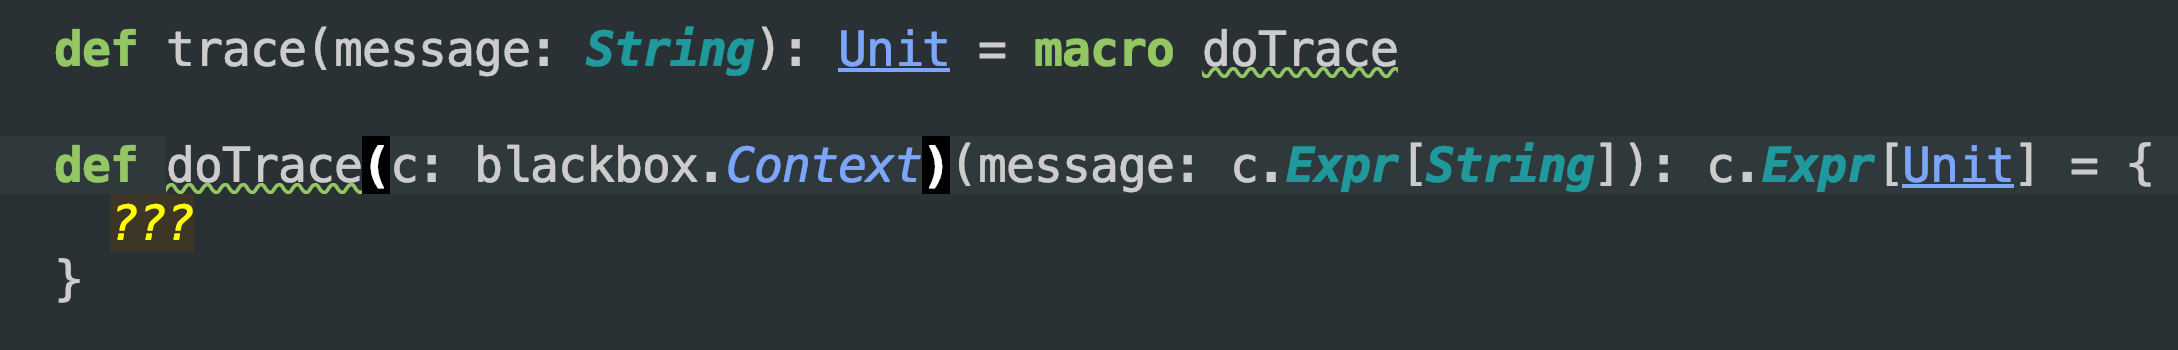
\includegraphics[width=\textwidth]{media/macro-snippet.png}
\end{figure}
\end{frame}

\section{The implementation: logstage}

\begin{frame}
\begin{figure}
\Huge 
\color{RubineRed} L✪GSTAGE
\noindent
{\color{RubineRed} \rule{\linewidth}{1mm} }
\Large First-class logging framework for Scala
\end{figure}
\end{frame}

\begin{frame}
\frametitle{Quick overview}
\begin{itemize}
\item Almost no dependencies,
\item Compile-time structure and context extraction,
\item Console and file sinks out of the box, log rotation supported,
\item Asynchronous sink out of the box (single worker thread at the moment),
\item String and JSON rendering out of the box,
\item Automatic structure identifiers for JSON policy,
\item Modular -- you may implement your own sink, router, etc,
\item DI-ready, no singletons or classpath scanners,
\item \textbf{Method}-level granularity,
\item User-provided logging contexts,
\item Slf4J backend -- LogStage is a drop-in replacement for Logback, route your legacy logs,
\item Location hyperlinks for IntelliJ console.
\end{itemize}
\end{frame}

\begin{frame}
\frametitle{An example}
\scalacode{target/ex-scala-logstage.tmp}
Followed by a cute screenshot of course:
\begin{figure}
    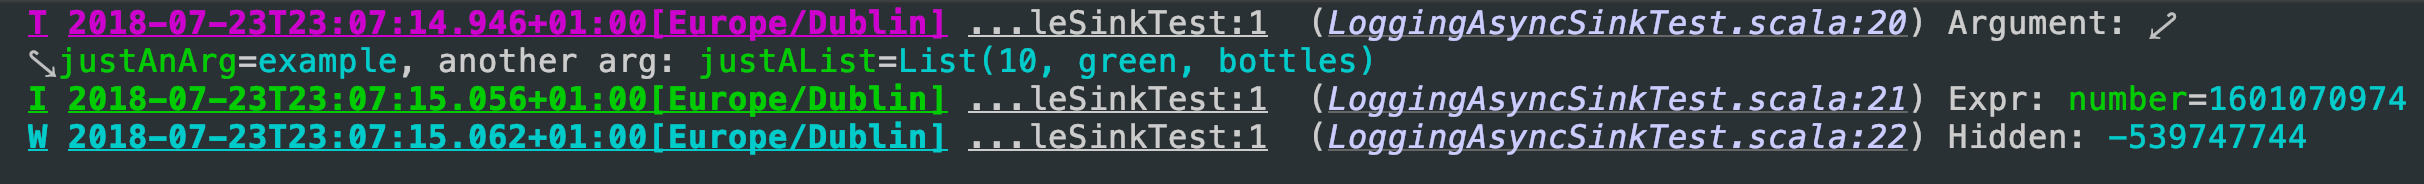
\includegraphics[width=\textwidth]{media/logstage-console.png}
\end{figure}
\end{frame}

\begin{frame}
\frametitle{Something nice for our robots}
\begin{figure}
    \inputminted[fontsize=\scriptsize]{json}{target/ex-json-out.tmp}
\end{figure}
\end{frame}

\begin{frame}
\frametitle{Status and things to do}
LogStage is:
\begin{itemize}
\item ready to use,
\item in real production for 4 months.
\end{itemize}
\vspace{0.3cm}
Our plans:
\begin{itemize}
\item Declarative router config,
\item Start using log events to collect metrics (keep in mind, we have derived structure identifiers),
\item Cleanups and refactorings.
\end{itemize}
\end{frame}

\begin{frame}
    \frametitle{Thank you for your attention}

    \begin{center}
      https://izumi.7mind.io/

      We're looking for clients, contributors, adopters and colleagues ;)
    \end{center}

    About the author:
    \begin{itemize}
        \item coding for 18 years, 10 years of hands-on commercial engineering experience,
        \item has been leading a cluster orchestration team in Yandex, ``the Russian Google'',
        \item implemented ``\textit{Interstellar Spaceship}'' -- an orchestration solution to manage 50K+ physical machines across 6 datacenters,
        \item Owns an Irish R\&D company, https://7mind.io,
        \item Contacts: team@7mind.io,
        \item Github: https://github.com/pshirshov
    \end{itemize}
\end{frame}

\end{document}
